
\section{Datasets, simulation samples and theoretical predictions}

%\subsection{Data}

\subsection{Triggers and Datasets}
\label{sec:trigpaths}


This analysis uses a ultra legacy data sample recorded by the CMS experiment during 2016, 2017 and 2018, corresponding to $\usedLumiABC$ of data.  
%The HLT paths used for different periods of collision data are listed in Table~\ref{tab:triggerPathsA},~\ref{tab:triggerPathsB}, and ~\ref{tab:triggerPathsC}. 

The datasets used for 2016, 2017 and 2018 data taking are listed in Tables~\ref{tab:datasets_dataA},~\ref{tab:datasets_dataB}, and~\ref{tab:datasets_dataC}, respectively, along with the integrated luminosity. 
%The datasets used are listed in Table~\ref{tab:datasets_dataC}. 
The analysis relies on four different primary datasets (PDs), {\it DoubleMuon}, {\it MuEG}, {\it EGamma} (or {\it DoubleEG} and {\it SingleElectron} for 2016 and 2017), and {\it SingleMuon},
each of which combines a certain collections of HLT paths. 
To avoid duplicate events from different primary datasets, events are taken: 
\begin{itemize}
\item from EGamma if they pass the diEle or triEle or singleElectron triggers,
\item from DoubleMuon if they pass the diMuon or triMuon triggers and fail the diEle and triEle triggers,
\item from MuEG if they pass the MuEle or MuDiEle or DiMuEle triggers and fail the diEle, triEle, singleElectron, diMuon and triMuon triggers,
%\item from SingleElectron if they pass the singleElectron trigger and fail all the above triggers. 
\item from SingleMuon if they pass the singleMuon trigger and fail all the above triggers. 
\end{itemize} 

The HLT paths used for 2016, 2017 and 2018 collision data are listed in Tables~\ref{tab:triggerPathsA},~\ref{tab:triggerPathsB} and~\ref{tab:triggerPathsC}, respectively.

\begin{table}[h]
	%\scriptsize
        \tiny
	\centering
	\begin{tabular}{|l|l|l|} 
		\hline %----------------------------------------------------------------------------------------
		\hline %---------------------------------------------------------------------------------------- 
		Run-range & Dataset & Integrated luminosity \\
		\hline %----------------------------------------------------------------------------------------
		\hline %---------------------------------------------------------------------------------------- 
		\multirow{5}{*}{272007-275376} & /DoubleMuon/Run2016C-21Feb2020\_UL2016\_HIPM-v1/MINIAOD &  \multirow{5}{*}{$5.892\ \text{fb}^{-1}$} \\ 
		& /DoubleMuon/Run2016B-21Feb2020\_ver1\_UL2016\_HIPM-v1/MINIAOD &  \\ 
		& /MuonEG/Run2016B-21Feb2020\_ver1\_UL2016\_HIPM-v1/MINIAOD &  \\ 
		& /SingleElectron/Run2016B-21Feb2020\_ver1\_UL2016\_HIPM-v1/MINIAOD &  \\ 
		& /SingleMuon/Run2016B-21Feb2020\_ver1\_UL2016\_HIPM-v1/MINIAOD &  \\ 
		\hline
		\multirow{5}{*}{275657-276283} & /DoubleMuon/Run2016C-17Jul2018-v1/MINIAOD &  \multirow{5}{*}{$2.646\ \text{fb}^{-1}$}  \\ 
		& /DoubleEG/Run2016C-21Feb2020\_UL2016\_HIPM-v1/MINIAOD &  \\ 
		& /MuonEG/Run2016C-21Feb2020\_UL2016\_HIPM-v1/MINIAOD &  \\ 
		& /SingleElectron/Run2016C-21Feb2020\_UL2016\_HIPM-v1/MINIAOD &  \\ 
		& /SingleMuon/Run2016C-21Feb2020\_UL2016\_HIPM-v1/MINIAOD &  \\ 
		\hline
		\multirow{5}{*}{276315-276811} & /DoubleEG/Run2016D-21Feb2020\_UL2016\_HIPM-v1/MINIAOD &  \multirow{5}{*}{$4.353\ \text{fb}^{-1}$} \\ 
		& /DoubleMuon/Run2016D-21Feb2020\_UL2016\_HIPM-v1/MINIAOD &  \\ 
		& /MuonEG/Run2016D-21Feb2020\_UL2016\_HIPM-v1/MINIAOD &  \\ 
		& /SingleElectron/Run2016D-21Feb2020\_UL2016\_HIPM-v1/MINIAOD &  \\ 
		& /SingleMuon/Run2016D-21Feb2020\_UL2016\_HIPM-v1/MINIAOD &  \\ 
		\hline
		\multirow{5}{*}{276831-277420} & /DoubleEG/Run2016E-21Feb2020\_UL2016\_HIPM-v1/MINIAOD &  \multirow{5}{*}{$4.117\ \text{fb}^{-1}$} \\ 
		& /DoubleMuon/Run2016E-21Feb2020\_UL2016\_HIPM-v1/MINIAOD &  \\ 
		& /MuonEG/Run2016E-21Feb2020\_UL2016\_HIPM-v1/MINIAOD &  \\ 
          	& /SingleElectron/Run2016E-21Feb2020\_UL2016\_HIPM-v1/MINIAOD &  \\ 
		& /SingleMuon/Run2016E-21Feb2020\_UL2016\_HIPM-v1/MINIAOD &  \\ 
		\hline
		\multirow{5}{*}{277772-278808} & /DoubleEG/Run2016F-21Feb2020\_UL2016-v1/MINIAOD &  \multirow{5}{*}{$3.186\ \text{fb}^{-1}$} \\ 
		& /DoubleMuon/Run2016F-21Feb2020\_UL2016\_HIPM-v1/MINIAOD &  \\ 
		& /MuonEG/Run2016F-21Feb2020\_UL2016-v1/MINIAOD &  \\ 
		& /SingleElectron/Run2016F-21Feb2020\_UL2016-v1/MINIAOD &  \\ 
		& /SingleMuon/Run2016F-21Feb2020\_UL2016-v1/MINIAOD &  \\ 
		\hline
		\multirow{5}{*}{278820-280385} & /DoubleEG/Run2016G-21Feb2020\_UL2016-v1/MINIAOD &  \multirow{5}{*}{$7.721\ \text{fb}^{-1}$} \\ 
		& /DoubleMuon/Run2016G-21Feb2020\_UL2016-v1/MINIAOD &  \\ 
		& /MuonEG/Run2016G-21Feb2020\_UL2016-v1/MINIAOD &  \\ 
		& /SingleElectron/Run2016G-21Feb2020\_UL2016-v1/MINIAOD &  \\ 
		& /SingleMuon/Run2016G-21Feb2020\_UL2016-v1/MINIAOD &  \\ 
		\hline
		%\multirow{15}{*}{280919-284044} & /DoubleEG/Run2016H-21Feb2020\_UL2016-v1/MINIAOD &  \multirow{15}{*}{$8.857\ \text{fb}^{-1}$} \\ 
		\multirow{5}{*}{280919-284044} & /DoubleEG/Run2016H-21Feb2020\_UL2016-v1/MINIAOD &  \multirow{5}{*}{$8.857\ \text{fb}^{-1}$} \\ 
		& /DoubleMuon/Run2016H-21Feb2020\_UL2016-v1/MINIAOD &  \\ 
		& /MuonEG/Run2016H-21Feb2020\_UL2016-v1/MINIAOD &  \\ 
		& /SingleElectron/Run2016H-21Feb2020\_UL2016-v2/MINIAOD &  \\ 
		& /SingleMuon/Run2016H-21Feb2020\_UL2016-v1/MINIAOD &  \\ 
%		& /DoubleMuon/Run2016H-17Jul2018-v1/MINIAOD &  \\ 
%		& /DoubleEG/Run2016H-17Jul2018-v1/MINIAOD &  \\ 
%		& /MuonEG/Run2016H-17Jul2018-v1/MINIAOD &  \\ 
%		& /SingleElectron/Run2016H-17Jul2018-v1/MINIAOD &  \\ 
%		& /SingleMuon/Run2016H-17Jul2018-v1/MINIAOD &  \\ 
%		& /DoubleMuon/Run2016H-17Jul2018-v1/MINIAOD &  \\ 
%		& /DoubleEG/Run2016H-17Jul2018-v1/MINIAOD &  \\ 
%		& /MuonEG/Run2016H-17Jul2018-v1/MINIAOD &  \\ 
%	        & /SingleElectron/Run2016H-17Jul2018-v1/MINIAOD &  \\ 
%		& /SingleMuon/Run2016H-17Jul2018-v1/MINIAOD &  \\ 
		\hline %----------------------------------------------------------------------------------------
		\hline %----------------------------------------------------------------------------------------
	\end{tabular}
	\small
	\caption{ Datasets used in the 2016 analysis. }
	\label{tab:datasets_dataA}
\end{table}


\begin{table}[h]
	%\scriptsize
        \tiny
	\centering
	\begin{tabular}{|l|l|c|l|} 
		\hline %--------------------------------------------------------------------------------------------------------------------------
		HLT path                      				                               & prescale  & primary dataset \\
		\hline %--------------------------------------------------------------------------------------------------------------------------
		\verb| HLT_Ele17_Ele12_CaloIdL_TrackIdL_IsoVL_DZ         |  & 1 & DoubleEG \\
		\verb| HLT_Ele23_Ele12_CaloIdL_TrackIdL_IsoVL_DZ         |  & 1 & DoubleEG \\
		\verb| HLT_DoubleEle33_CaloIdL_GsfTrkIdVL                |  & 1 & DoubleEG \\
		\verb| HLT_Ele16_Ele12_Ele8_CaloIdL_TrackIdL             |  & 1 & DoubleEG \\
		\verb| HLT_Mu17_TrkIsoVVL_Mu8_TrkIsoVVL                  |  & 1 & DoubleMuon \\
		\verb| HLT_Mu17_TrkIsoVVL_TkMu8_TrkIsoVVL                |  & 1 & DoubleMuon \\
		\verb| HLT_TripleMu_12_10_5                              |  & 1 & DoubleMuon \\
		\verb| HLT_Mu8_TrkIsoVVL_Ele17_CaloIdL_TrackIdL_IsoVL    |  & 1 & MuonEG \\
		\verb| HLT_Mu8_TrkIsoVVL_Ele23_CaloIdL_TrackIdL_IsoVL    |  & 1 & MuonEG \\
		\verb| HLT_Mu17_TrkIsoVVL_Ele12_CaloIdL_TrackIdL_IsoVL   |  & 1 & MuonEG \\
		\verb| HLT_Mu23_TrkIsoVVL_Ele12_CaloIdL_TrackIdL_IsoVL   |  & 1 & MuonEG \\
		\verb| HLT_Mu23_TrkIsoVVL_Ele8_CaloIdL_TrackIdL_IsoVL    |  & 1 & MuonEG \\
		\verb| HLT_Mu8_DiEle12_CaloIdL_TrackIdL                  |  & 1 & MuonEG \\
		\verb| HLT_DiMu9_Ele9_CaloIdL_TrackIdL                   |  & 1 & MuonEG \\
		\verb| HLT_Ele25_eta2p1_WPTight                          |  & 1 & SingleElectron \\
		\verb| HLT_Ele27_WPTight                                 |  & 1 & SingleElectron \\
		\verb| HLT_Ele27_eta2p1_WPLoose_Gsf                      |  & 1 & SingleElectron \\
		\verb| HLT_IsoMu20 OR HLT_IsoTkMu20                      |  & 1 & SingleMuon \\
		\verb| HLT_IsoMu22 OR HLT_IsoTkMu22                      |  & 1 & SingleMuon \\
		\hline %--------------------------------------------------------------------------------------------------------------------------
	\end{tabular}
	\small
	\caption{Trigger paths used in 2016 collision data.}
	\label{tab:triggerPathsA}
\end{table}

\begin{table}[h]
\scriptsize
    \centering
    \begin{tabular}{|l|l|l|} 
\hline %----------------------------------------------------------------------------------------
\hline %---------------------------------------------------------------------------------------- 
Run-range & Dataset & Integrated luminosity \\
\hline %----------------------------------------------------------------------------------------
\hline %---------------------------------------------------------------------------------------- 
\multirow{5}{*}{297046-299329} & /DoubleMuon/Run2017B-UL2017\_MiniAODv2-v1/MINIAOD &  \multirow{5}{*}{$4.792\ \text{fb}^{-1}$} \\ 
& /DoubleEG/Run2017B-09Aug2019\_UL2017-v1/MINIAOD &  \\ 
& /MuonEG/Run2017B-UL2017\_MiniAODv2-v1/MINIAOD &  \\ 
& /SingleElectron/Run2017B-UL2017\_MiniAODv2-v1/MINIAOD &  \\ 
& /SingleMuon/Run2017B-09Aug2019\_UL2017-v1/MINIAOD &  \\ 
\hline
\multirow{5}{*}{299368-300676} & /DoubleMuon/Run2017C-UL2017\_MiniAODv2-v1/MINIAOD &  \multirow{5}{*}{$9.755\ \text{fb}^{-1}$}  \\ 
& /DoubleEG/Run2017C-UL2017\_MiniAODv2-v2/MINIAOD &  \\ 
& /MuonEG/Run2017C-UL2017\_MiniAODv2-v1/MINIAOD &  \\ 
& /SingleElectron/Run2017C-UL2017\_MiniAODv2-v1/MINIAOD &  \\ 
& /SingleMuon/Run2017C-09Aug2019\_UL2017-v1/MINIAOD &  \\ 
\hline
%%\multirow{5}{*}{300742-302029} & /DoubleMuon/Run2017C-17Nov2017-v1/MINIAOD &  \multirow{5}{*}{$9.755\ \text{fb}^{-1}$}  \\ 
%%& /DoubleEG/Run2017C-17Nov2017-v1/MINIAOD &  \\ 
%%& /MuonEG/Run2017C-17Nov2017-v1/MINIAOD &  \\ 
%%& /SingleElectron/Run2017C-17Nov2017-v1/MINIAOD &  \\ 
%%& /SingleMuon/Run2017C-17Nov2017-v1/MINIAOD &  \\ 
%%\hline
\multirow{5}{*}{302030-303434} & /DoubleMuon/Run2017D-UL2017\_MiniAODv2-v1/MINIAOD &  \multirow{5}{*}{$4.319\ \text{fb}^{-1}$} \\ 
& /DoubleEG/Run2017D-UL2017\_MiniAODv2-v1/MINIAOD &  \\ 
& /MuonEG/Run2017D-UL2017\_MiniAODv2-v1/MINIAOD &  \\ 
& /SingleElectron/Run2017D-09Aug2019\_UL2017-v1/MINIAOD &  \\ 
& /SingleMuon/Run2017D-09Aug2019\_UL2017-v1/MINIAOD &  \\ 
\hline
\multirow{5}{*}{303824-304797} & /DoubleMuon/Run2017E-09Aug2019\_UL2017-v1/MINIAOD &  \multirow{5}{*}{$9.424\ \text{fb}^{-1}$} \\ 
& /DoubleEG/Run2017E-UL2017\_MiniAODv2-v1/MINIAOD &  \\ 
& /MuonEG/Run2017E-UL2017\_MiniAODv2-v1/MINIAOD &  \\ 
& /SingleElectron/Run2017E-UL2017\_MiniAODv2-v1/MINIAOD &  \\ 
& /SingleMuon/Run2017E-09Aug2019\_UL2017-v1/MINIAOD &  \\ 
\hline
\multirow{5}{*}{305040-306462} & /DoubleMuon/Run2017F-UL2017\_MiniAODv2-v1/MINIAOD &  \multirow{5}{*}{$13.50\ \text{fb}^{-1}$} \\ 
& /DoubleEG/Run2017F-09Aug2019\_UL2017-v1/MINIAOD &  \\ 
& /MuonEG/Run2017F-UL2017\_MiniAODv2-v1/MINIAOD &  \\ 
& /SingleElectron/Run2017F-UL2017\_MiniAODv2-v1/MINIAOD &  \\ 
& /SingleMuon/Run2017F-09Aug2019\_UL2017-v1/MINIAOD &  \\ 
\hline
\multirow{5}{*}{278820-280385} & /DoubleMuon/Run2017G-09Aug2019\_UL2017-v1/MINIAOD &  \multirow{5}{*}{$7.721\ \text{fb}^{-1}$} \\ 
 & /DoubleEG/Run2017G??/MINIAOD &  \\ 
 & /MuonEG/Run2017G??/MINIAOD &  \\ 
 & /SingleElectron/Run2017G??/MINIAOD &  \\ 
 & /SingleMuon/Run2017G?/MINIAOD &  \\ 
 \hline
 %\multirow{15}{*}{281207-284068} & /DoubleMuon/Run2017H-UL2017\_MiniAODv2-v1/MINIAOD &  \multirow{15}{*}{$8.857\ \text{fb}^{-1}$} \\ 
 \multirow{5}{*}{281207-284068} & /DoubleMuon/Run2017H-UL2017\_MiniAODv2-v1/MINIAOD &  \multirow{5}{*}{$8.857\ \text{fb}^{-1}$} \\ 
 & /DoubleEG/Run2017??/MINIAOD &  \\ 
 & /MuonEG/Run2017H??/MINIAOD &  \\ 
 & /SingleElectron/Run2017H??/MINIAOD &  \\ 
 & /SingleMuon/Run2017H??/MINIAOD &  \\ 
% & /DoubleMuon/Run2017H-PromptReco-v2/MINIAOD &  \\ 
% & /DoubleEG/Run2017H-PromptReco-v2/MINIAOD &  \\ 
% & /MuonEG/Run2017H-PromptReco-v2/MINIAOD &  \\ 
% & /SingleElectron/Run2017H-PromptReco-v2/MINIAOD &  \\ 
% & /SingleMuon/Run2017H-PromptReco-v2/MINIAOD &  \\ 
% & /DoubleMuon/Run2017H-PromptReco-v3/MINIAOD &  \\ 
% & /DoubleEG/Run2017H-PromptReco-v3/MINIAOD &  \\ 
% & /MuonEG/Run2017H-PromptReco-v3/MINIAOD &  \\ 
% & /SingleElectron/Run2017H-PromptReco-v3/MINIAOD &  \\ 
% & /SingleMuon/Run2017H-PromptReco-v3/MINIAOD &  \\ 
\hline %----------------------------------------------------------------------------------------
\hline %----------------------------------------------------------------------------------------
     \end{tabular}
\small
    \caption{ Datasets used in the 2017 analysis. }
    \label{tab:datasets_dataB}
\end{table}


\begin{table}[h]
\scriptsize
    \centering
    \begin{tabular}{|l|l|c|l|} 
\hline %--------------------------------------------------------------------------------------------------------------------------
HLT path                      				                               & prescale  & primary dataset \\
\hline %--------------------------------------------------------------------------------------------------------------------------
\verb| HLT_Ele23_Ele12_CaloIdL_TrackIdL_IsoVL_*           |  & 1 & DoubleEG \\
\verb| HLT_DoubleEle33_CaloIdL_GsfTrkIdVL                 |  & 1 & DoubleEG \\
\verb| HLT_Ele16_Ele12_Ele8_CaloIdL_TrackIdL              |  & 1 & DoubleEG \\
\verb| HLT_Mu17_TrkIsoVVL_Mu8_TrkIsoVVL_DZ_Mass3p8        |  & 1 & DoubleMuon \\
\verb| HLT_Mu17_TrkIsoVVL_Mu8_TrkIsoVVL_DZ_Mass8          |  & 1 & DoubleMuon \\
\verb| HLT_TripleMu_12_10_5                               |  & 1 & DoubleMuon \\
\verb| HLT_TripleMu_10_5_5_D2                             |  & 1 & DoubleMuon \\
\verb| HLT_Mu23_TrkIsoVVL_Ele12_CaloIdL_TrackIdL_IsoVL    | & 1 & MuonEG \\
\verb| HLT_Mu8_TrkIsoVVL_Ele23_CaloIdL_TrackIdL_IsoVL_DZ  | & 1 & MuonEG \\
\verb| HLT_Mu12_TrkIsoVVL_Ele23_CaloIdL_TrackIdL_IsoVL_DZ | & 1 & MuonEG \\
\verb| HLT_Mu23_TrkIsoVVL_Ele12_CaloIdL_TrackIdL_IsoVL_DZ | & 1 & MuonEG \\
\verb| HLT_DiMu9_Ele9_CaloIdL_TrackIdL_DZ                 | & 1 & MuonEG \\
\verb| HLT_Mu8_DiEle12_CaloIdL_TrackIdL                   | & 1 & MuonEG \\
\verb| HLT_Mu8_DiEle12_CaloIdL_TrackIdL_DZ                | & 1 & MuonEG \\
\verb| HLT_Ele35_WPTight_Gsf_v*                           | & 1 & SingleElectron \\
\verb| HLT_Ele38_WPTight_Gsf_v*                           | & 1 & SingleElectron \\
\verb| HLT_Ele40_WPTight_Gsf_v*                           | & 1 & SingleElectron \\
\verb| HLT_IsoMu27                                        | & 1 & SingleMuon \\
\hline %--------------------------------------------------------------------------------------------------------------------------
    \end{tabular}
\small
    \caption{Trigger paths used in 2017 collision data.  }
    \label{tab:triggerPathsB}
\end{table}



\begin{table}[h]
	\scriptsize
	\centering
	\begin{tabular}{|l|l|l|} 
		\hline %----------------------------------------------------------------------------------------
		\hline %---------------------------------------------------------------------------------------- 
		Run-range & Dataset & Integrated luminosity \\
		\hline %----------------------------------------------------------------------------------------
		\hline %---------------------------------------------------------------------------------------- 
		\multirow{5}{*}{315252-316995} & /DoubleMuon/Run2018A-UL2018\_MiniAODv2-v1/MINIAOD &  \multirow{5}{*}{$X.XXX\ \text{fb}^{-1}$} \\ 
		& /MuonEG/Run2018A-12Nov2019\_UL2018\_rsb-v1/MINIAOD &  \\ 
		& /EGamma/Run2018A-12Nov2019\_UL2018-v2/MINIAOD &  \\ 
		& /SingleMuon/Run2018A-UL2018\_MiniAODv2-v1/MINIAOD &  \\ 
		\hline
		\multirow{5}{*}{317080-319310} & /DoubleMuon/Run2018B-UL2018\_MiniAODv2-v2/MINIAOD &  \multirow{5}{*}{$X.XXX\ \text{fb}^{-1}$}  \\  
		& /MuonEG/Run2018B-12Nov2019\_UL2018-v1/MINIAOD &  \\ 
		& /EGamma/Run2018B-UL2018\_MiniAODv2-v1/MINIAOD &  \\ 
		& /SingleMuon/Run2018B-12Nov2019\_UL2018-v2/MINIAOD &  \\ 
		\hline
		\multirow{5}{*}{319337-320065} & /DoubleMuon/Run2018C-12Nov2019\_UL2018-v2/MINIAOD &  \multirow{5}{*}{$X.XXX\ \text{fb}^{-1}$} \\ 
		& /MuonEG/Run2018C-12Nov2019\_UL2018-v1/MINIAOD &  \\ 
		& /EGamma/Run2018C-UL2018\_MiniAODv2-v1/MINIAOD &  \\ 
		& /SingleMuon/Run2018C-12Nov2019\_UL2018-v2/MINIAOD &  \\ 
		\hline
		\multirow{5}{*}{320673-325175} & /DoubleMuon/Run2018D-UL2018\_MiniAODv2-v1/MINIAOD &  \multirow{5}{*}{$X.XXX\ \text{fb}^{-1}$} \\  
		& /MuonEG/Run2018D-12Nov2019\_UL2018\_rsb-v1/MINIAOD &  \\ 
		& /EGamma/Run2018D-UL2018\_MiniAODv2-v1/MINIAOD &  \\ 
		& /SingleMuon/Run2018D-12Nov2019\_UL2018-v4/MINIAOD &  \\ 
		\hline
		\hline
%		\hline %----------------------------------------------------------------------------------------
%		\hline %----------------------------------------------------------------------------------------
	\end{tabular}
	\small
	\caption{Datasets used in the 2018 analysis. }
	\label{tab:datasets_dataC}
\end{table}


\begin{table}[h]
	\scriptsize
	\centering
	\begin{tabular}{|l|c|l|} 
		\hline %--------------------------------------------------------------------------------------------------------------------------
		HLT path                      				       & prescale  & primary dataset \\
		\hline %--------------------------------------------------------------------------------------------------------------------------
		\verb| HLT_Ele23_Ele12_CaloIdL_TrackIdL_IsoVL_v*        | & 1 & DoubleEG \\
		\verb| HLT_DoubleEle25_CaloIdL_MW_v*              | & 1 & DoubleEG \\
		\verb| HLT_Mu17_TrkIsoVVL_Mu8_TrkIsoVVL_DZ_Mass3p8_v*     | & 1 & DoubleMuon \\
		\verb| HLT_Mu23_TrkIsoVVL_Ele12_CaloIdL_TrackIdL_IsoVL_v* | & 1 & MuonEG \\
		\verb| HLT_Mu8_TrkIsoVVL_Ele23_CaloIdL_TrackIdL_IsoVL_DZ_v* | & 1 & MuonEG \\
		\verb| HLT_Mu12_TrkIsoVVL_Ele23_CaloIdL_TrackIdL_IsoVL_DZ_v*| & 1 & MuonEG \\
		%\verb| HLT_Mu23_TrkIsoVVL_Ele12_CaloIdL_TrackIdL_IsoVL_DZ_v*| & 1 & MuonEG \\
		\verb| HLT_DiMu9_Ele9_CaloIdL_TrackIdL_DZ_v*| & 1 & MuonEG \\
		\verb| HLT_Ele32_WPTight_Gsf_v*                        | & 1 & SingleElectron \\
		\verb| HLT_IsoMu24_v*                                     | & 1 & SingleMuon \\
		\hline %--------------------------------------------------------------------------------------------------------------------------
	\end{tabular}
	\small
	\caption{Trigger paths used in 2018 collision data.  }
	\label{tab:triggerPathsC}
\end{table}

\clearpage 

\subsubsection{Trigger Efficiency}
%\textbf{FIX ME: TO BE UPDATED}

The efficiency in data of the combination of triggers used in the analysis with respect to the offline reconstruction and selection is measured
by considering 4$\ell$ events triggered by single lepton triggers. Details on the procedures are described in $\mathrm{H}\rightarrow{\rm Z}{\rm Z}\rightarrow4\ell$ ($\ell={\rm e},\mu$) analyses common note \cite{CMS-PAS-HIG-19-001}. 
%One of the four reconstructed leptons ( the ``tag'') is geometrically matched 
%to a trigger object passing the final filter of one of the single muon or single electron triggers. The other three leptons are 
%used as ``probes''. In each 4$\ell$ event there are up to 4 possible tag-probe combinations, and all possible combinations are counted in the
%denominator of the efficiency. For each of the three probe leptons all matching trigger filter objects are collected. Then the matched trigger filter
%objects of the three probe leptons are combined in attempt to reconstruct any of the triggers used in the analysis. If any of the analysis triggers
%can be formed using the probe leptons, the set of probes is also counted in the numerator of the efficiency.
%
%This method does not have a perfect closure in MC events due to the fact that the presence of a fourth lepton increases the trigger efficiency,
%and this effect is not accounted for. Also, in the  $2e2\mu$ final state, the three probe leptons cannot be combined to form all possible triggers which 
%can collect events with two electrons and two muons (e.g. if the tag lepton is an electron, the three remaining leptons cannot pass a double electron
%trigger). Therefore the method is also applied on MC and the difference between data and MC is used to determine the reliability of the simulation.
% The efficiency plotted as a function of the minimum $p_{\rm{T}}$ of the three probe leptons in data and MC using this method can be seen in 
%Fig.~\ref{fig:TrigEffC} that shows the trigger efficiency in 2018 data for different final states. The MC efficiency describes well the data within the statistical uncertainties.
%
%=======
%\begin{figure}[!htb]
%\vspace*{0.3cm}
%\begin{center}
%\includegraphics[width=0.45\textwidth]{Figures/Trigger/2016/Histo_TrigEff_ptMin_4e.pdf} 
%\includegraphics[width=0.45\textwidth]{Figures/Trigger/2016/Histo_TrigEff_ptMin_4mu.pdf} \\
%\includegraphics[width=0.45\textwidth]{Figures/Trigger/2016/Histo_TrigEff_ptMin_2e2mu.pdf} 
%\includegraphics[width=0.45\textwidth]{Figures/Trigger/2016/Histo_TrigEff_ptMin_4l.pdf} \\
%\caption{Trigger efficiency measured in 2016 data using $4\ell$ events collected by single lepton triggers for the $4e$ (top left), $4\mu$ (top right), $2e2\mu$ (bottom left) and $4\ell$ (bottom right) final states. 
%\label{fig:TrigEffA}}
%\end{center}
%\end{figure}
%=======

%=======
%\begin{figure}[!htb]
%	\vspace*{0.3cm}
%	\begin{center}
%		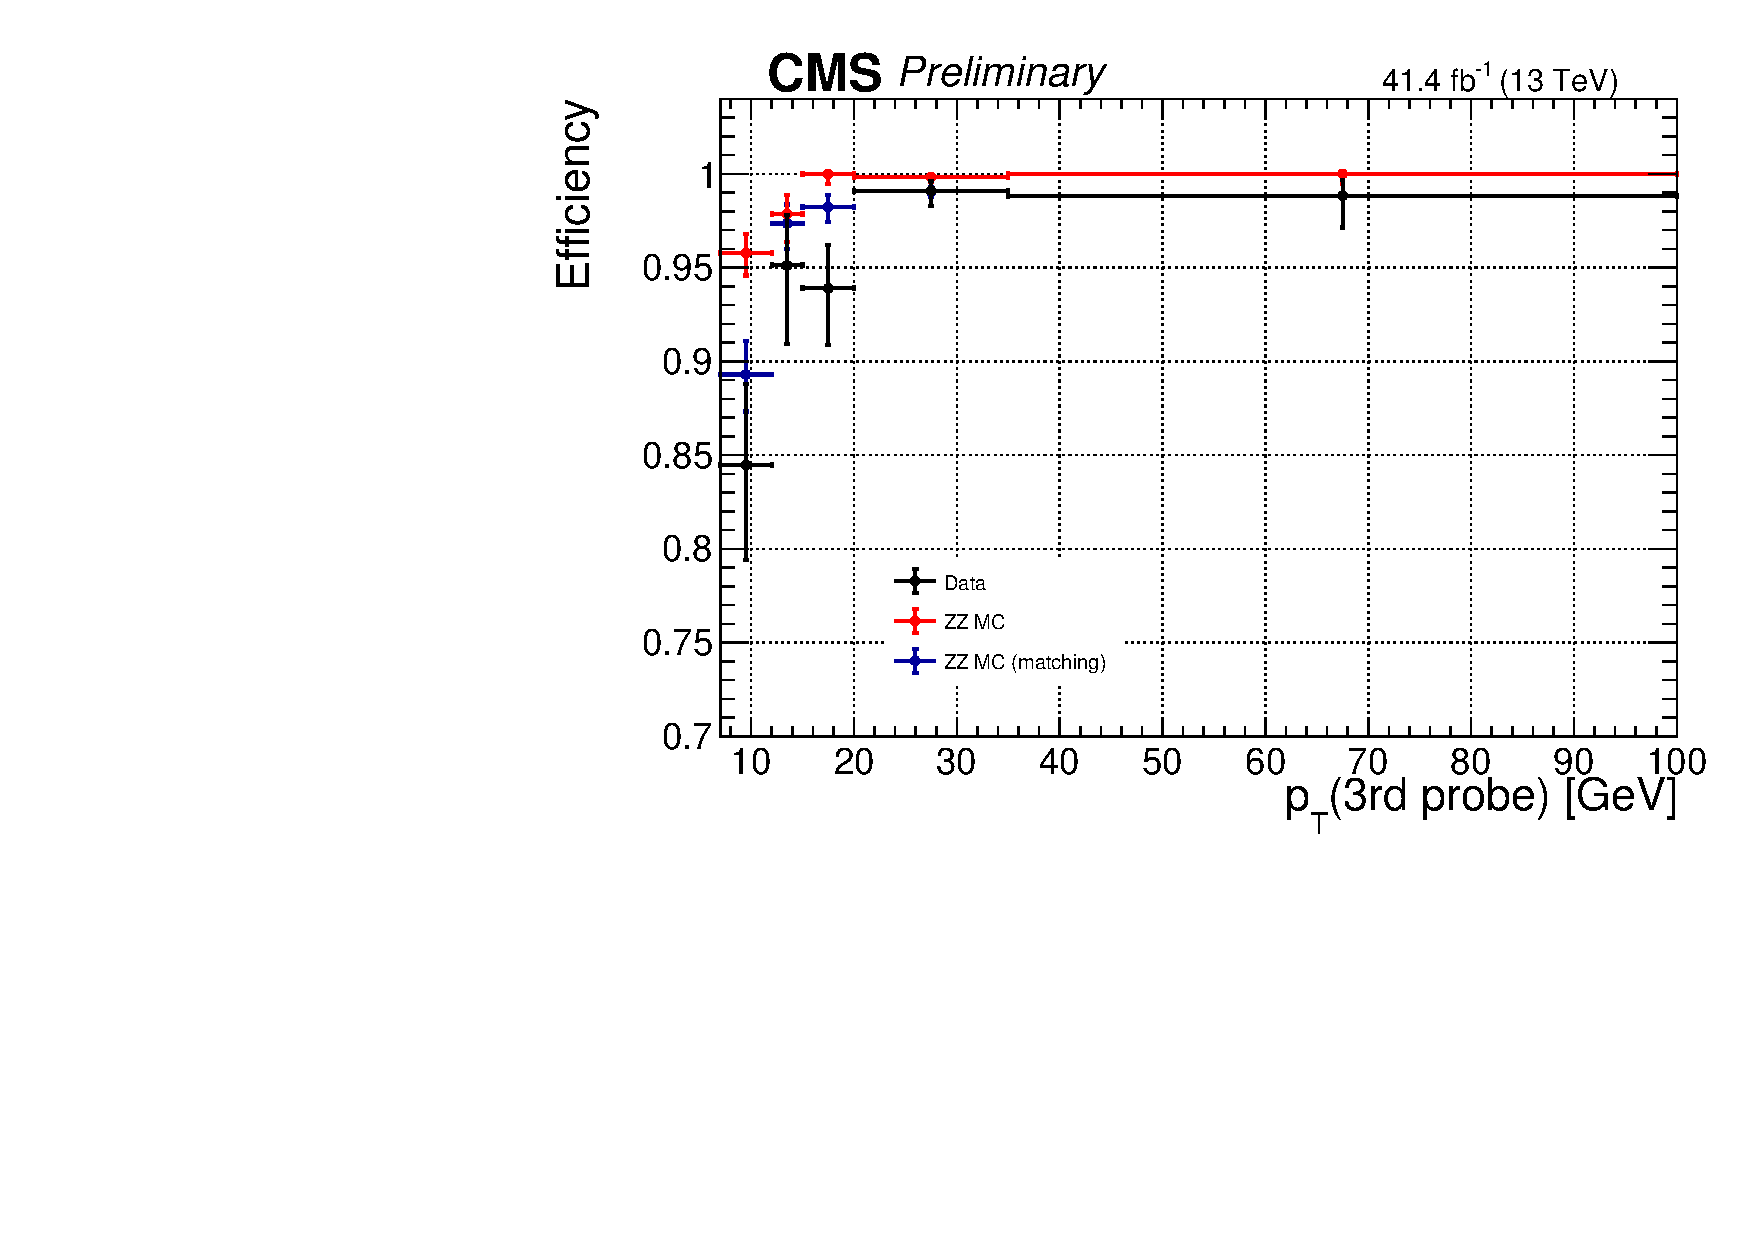
\includegraphics[width=0.45\textwidth]{Figures/Trigger/2017/Histo_TrigEff_ptMin_4e_mZ2_12.pdf} 
%		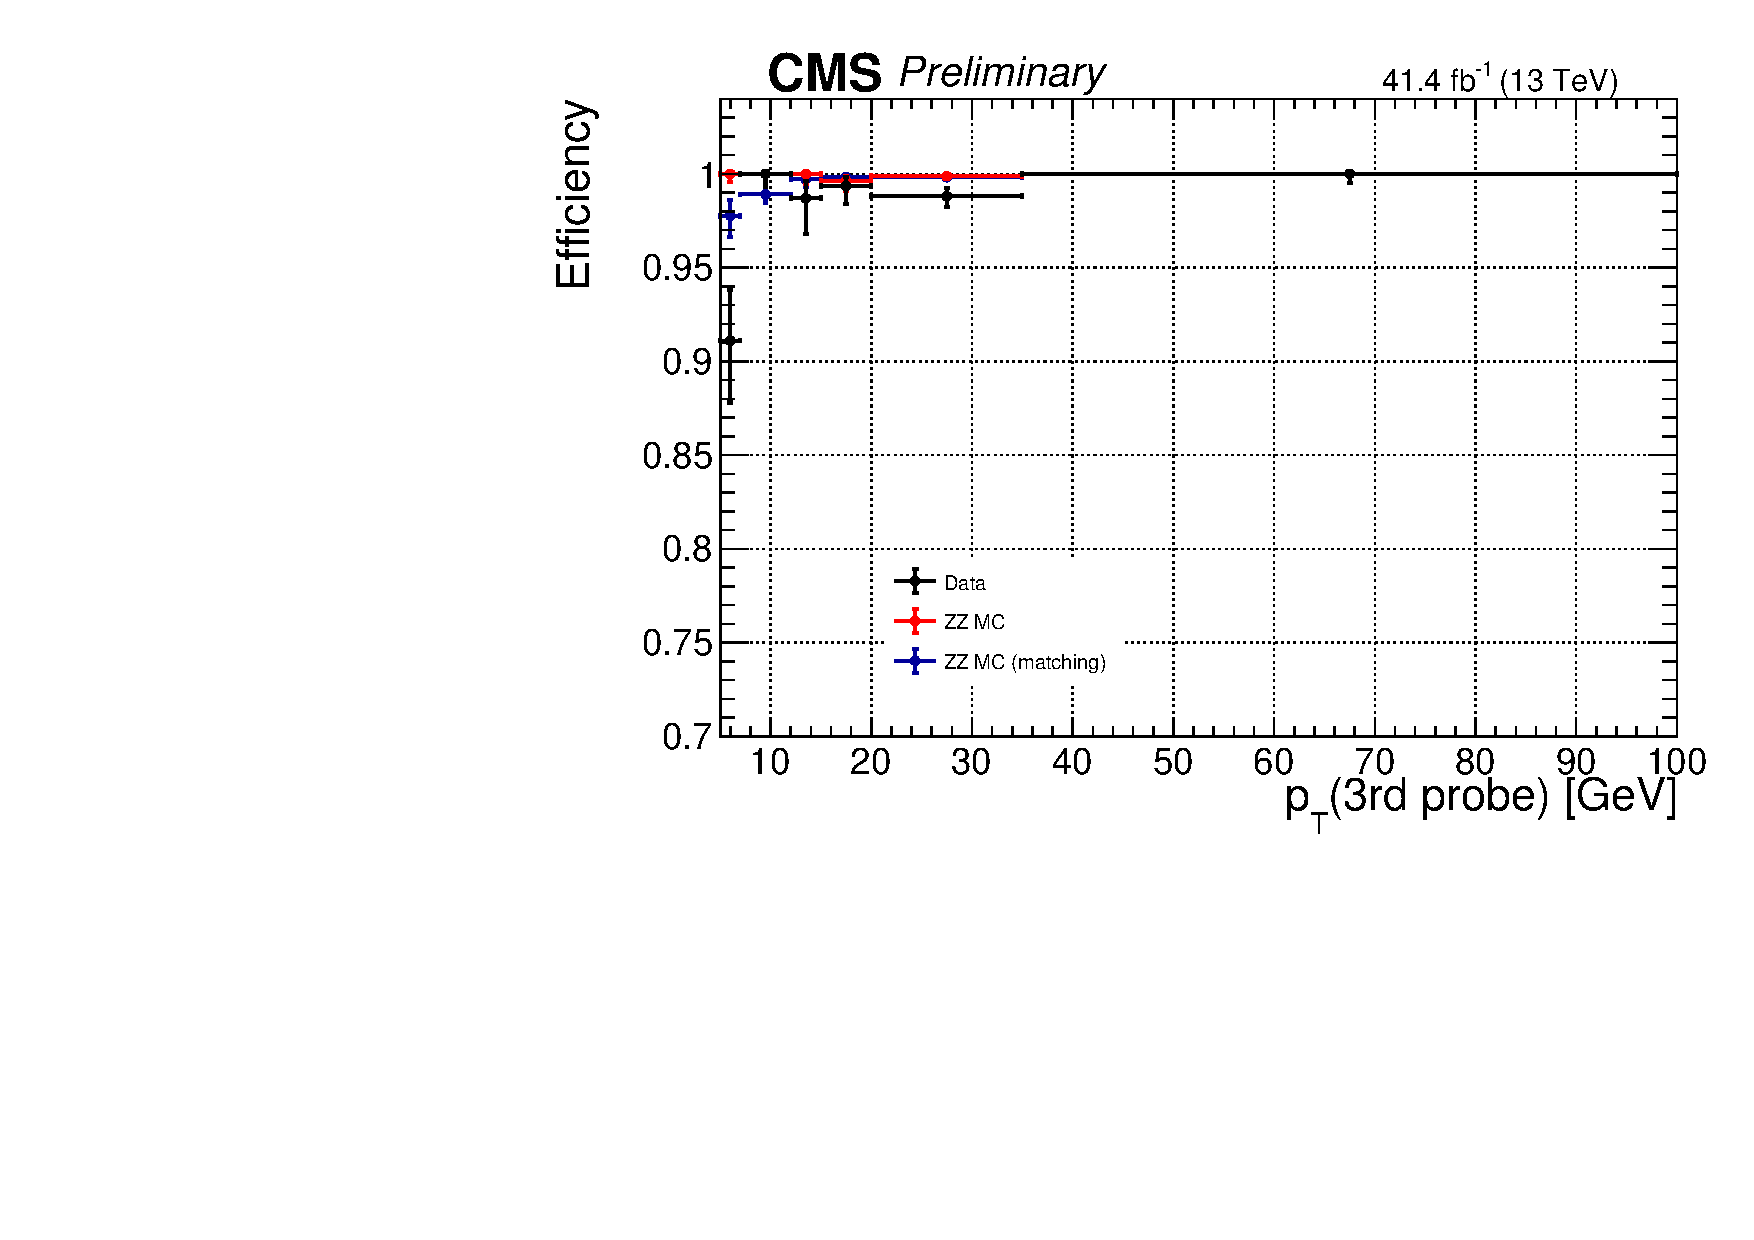
\includegraphics[width=0.45\textwidth]{Figures/Trigger/2017/Histo_TrigEff_ptMin_4mu_mZ2_12.pdf} \\
%		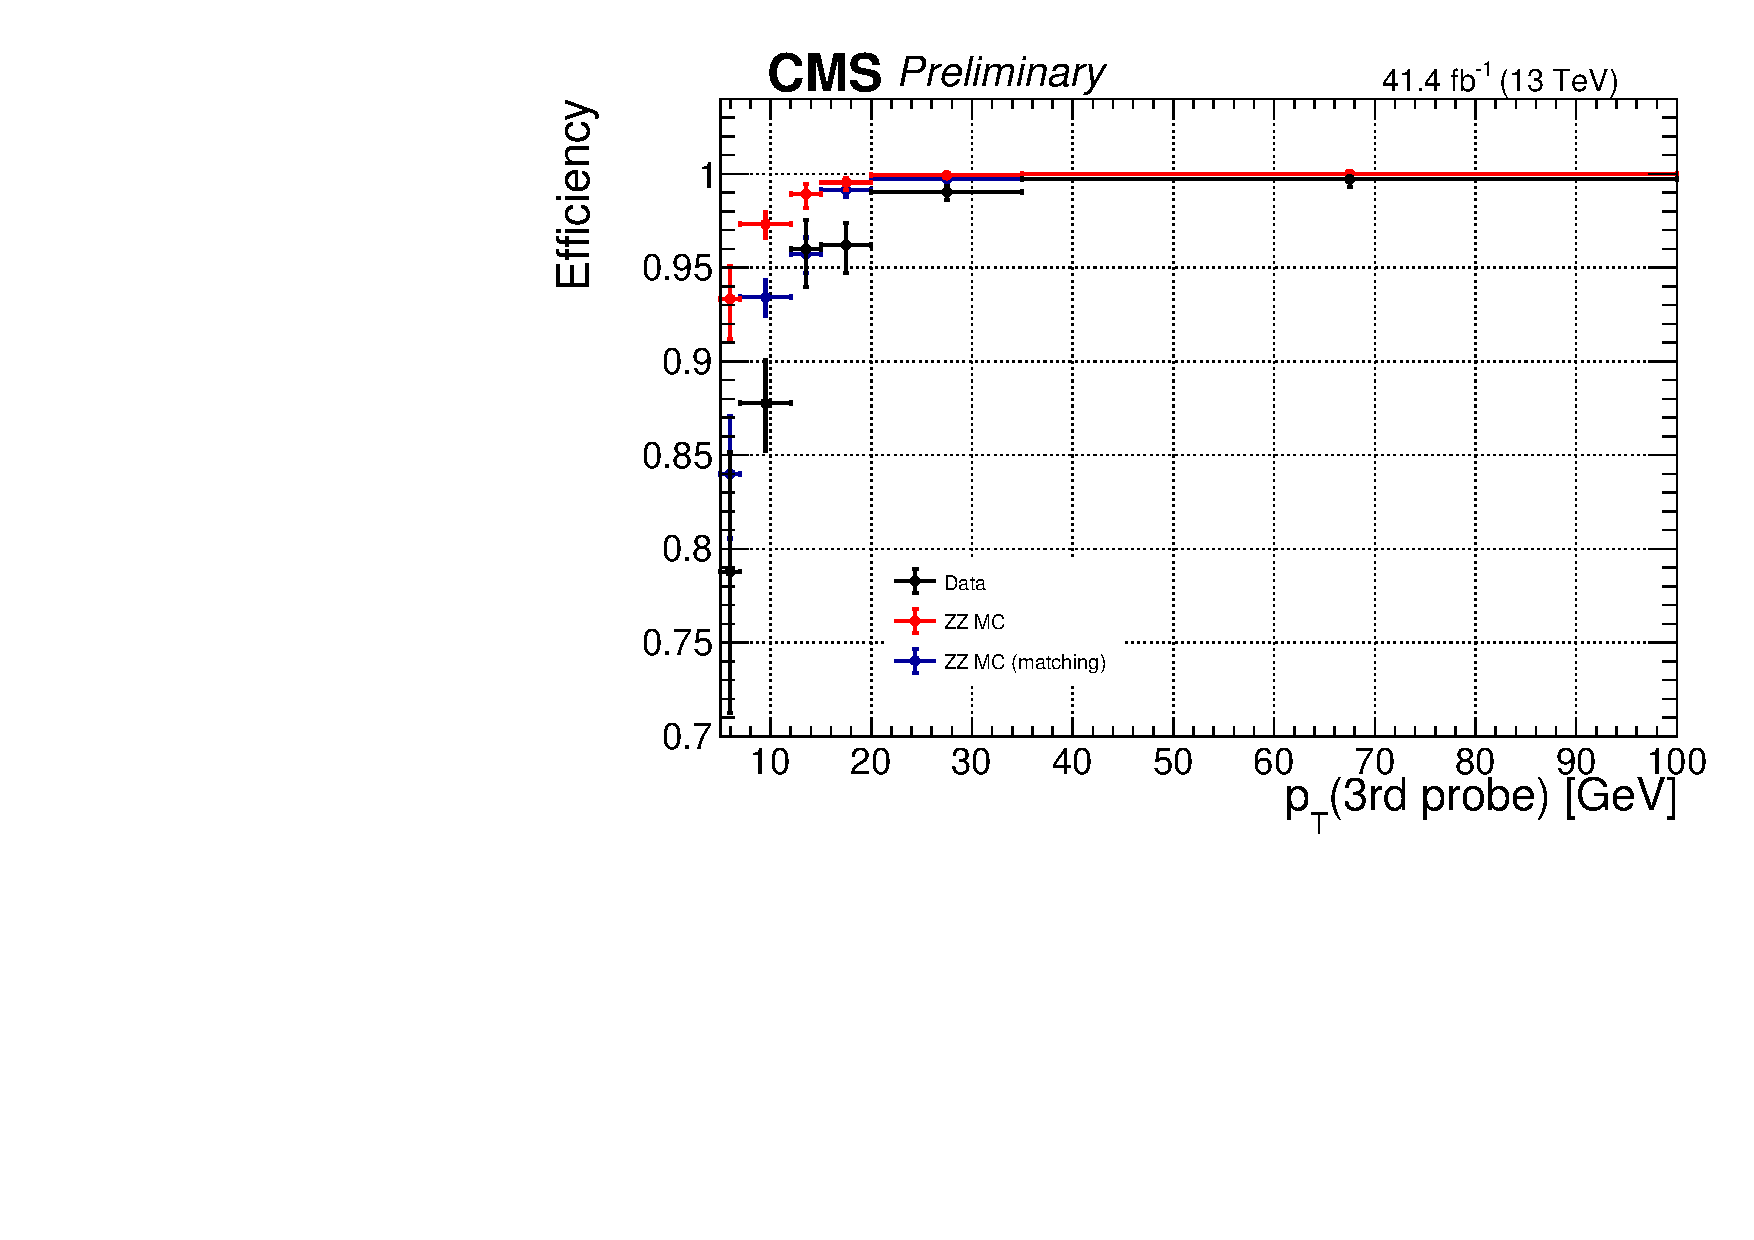
\includegraphics[width=0.45\textwidth]{Figures/Trigger/2017/Histo_TrigEff_ptMin_2e2mu_mZ2_12.pdf} 
%		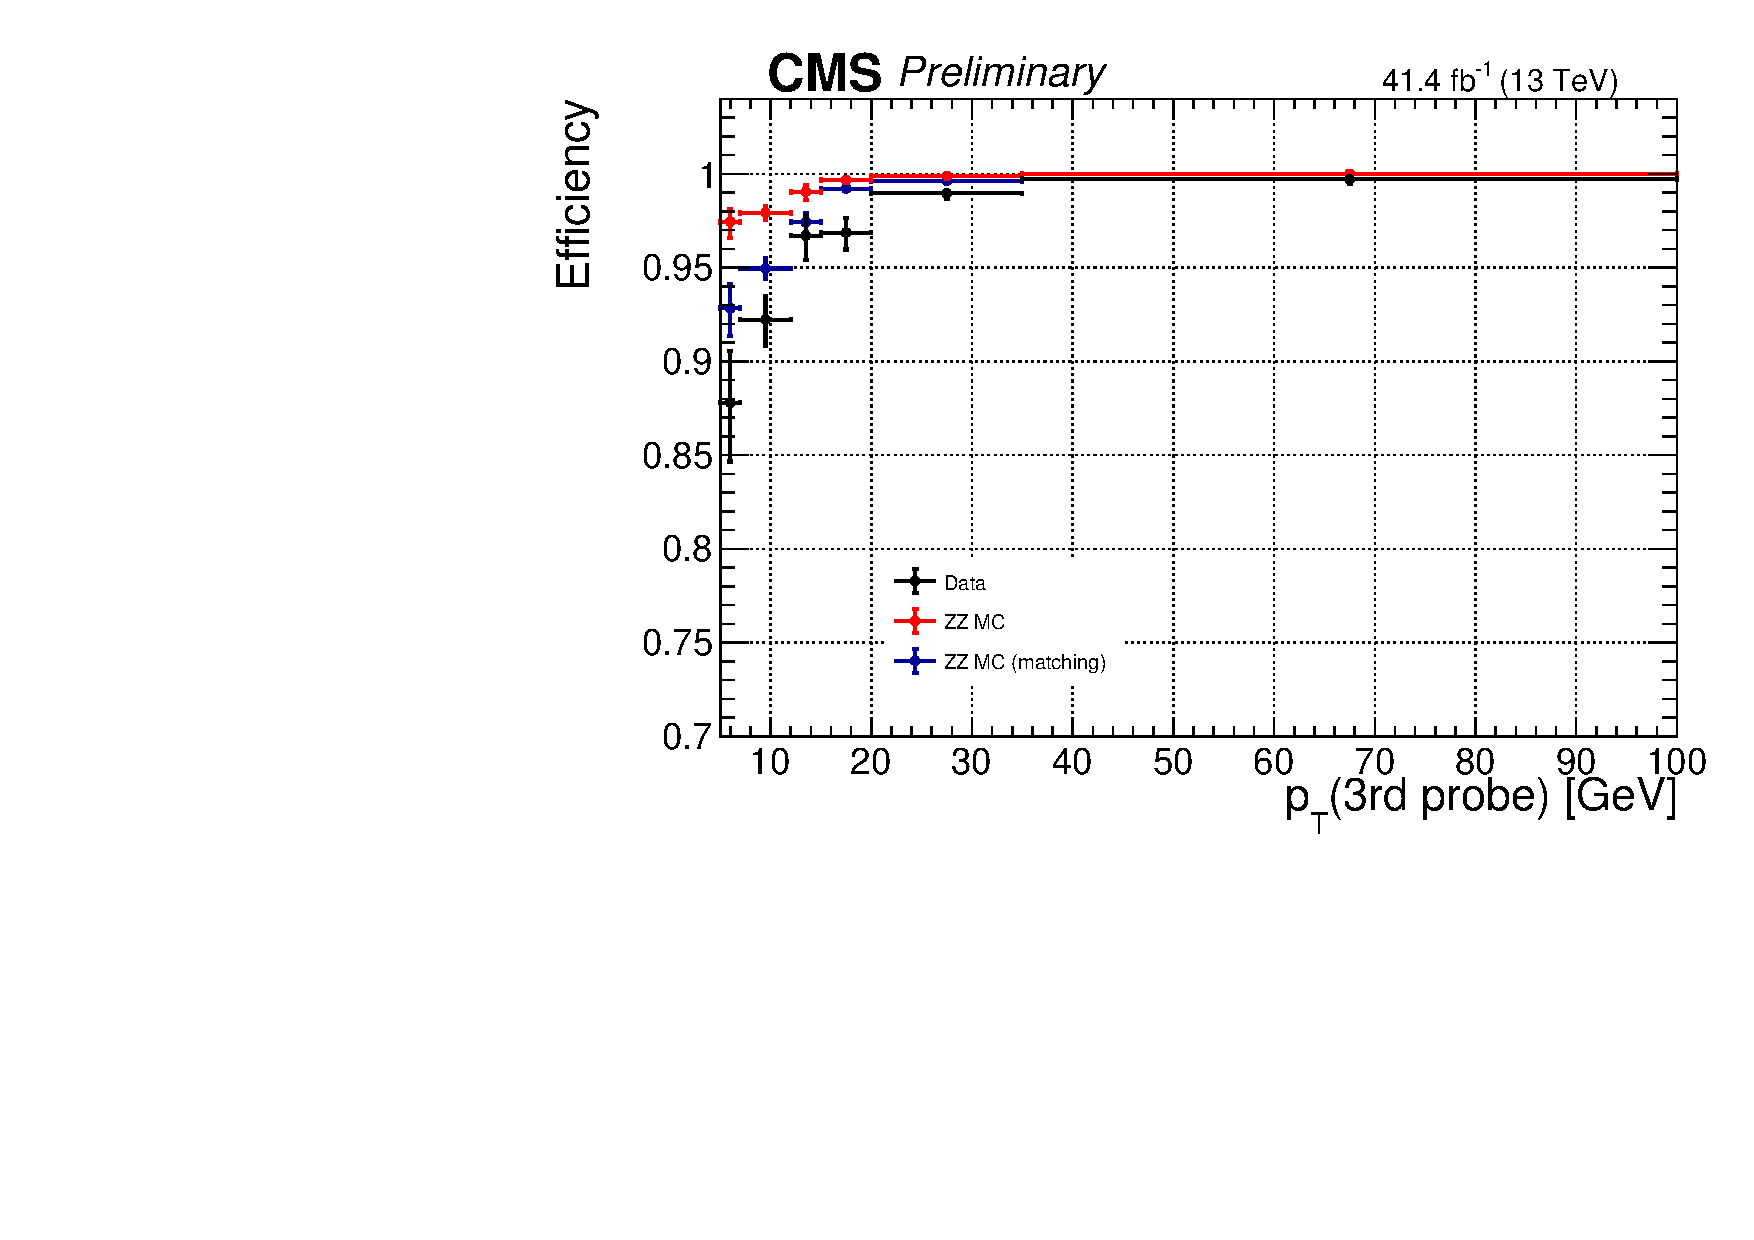
\includegraphics[width=0.45\textwidth]{Figures/Trigger/2017/Histo_TrigEff_ptMin_4l_mZ2_12.pdf} \\
%		\caption{Trigger efficiency measured in 2017 data using $4\ell$ events collected by single lepton triggers for the $4e$ (top left), $4\mu$ (top right), $2e2\mu$ (bottom left) and $4\ell$ (bottom right) final states. 
%			\label{fig:TrigEffB}}
%	\end{center}
%\end{figure}
%=======

%=======
%\begin{figure}[!htb]
%	\vspace*{0.3cm}
%	\begin{center}
%		\includegraphics[width=0.45\textwidth]{Figures/Trigger/Histo_TrigEff_ptMin_4e.pdf} 
%		\includegraphics[width=0.45\textwidth]{Figures/Trigger/Histo_TrigEff_ptMin_4mu.pdf} \\
%		\includegraphics[width=0.45\textwidth]{Figures/Trigger/Histo_TrigEff_ptMin_2e2mu.pdf} 
%		\includegraphics[width=0.45\textwidth]{Figures/Trigger/Histo_TrigEff_ptMin_4l.pdf} \\
%		\caption{ %\textbf{FIXME: Add figure once ready.}
%		Trigger efficiency measured in 2016 data using $4\ell$ events collected by single lepton triggers for the $4e$ (top left), $4\mu$ (top right), $2e2\mu$ (bottom left) and $4\ell$ (bottom right) final states. 
%			\label{fig:TrigEffC}}
%	\end{center}
%\end{figure}
%%=======

A summary of the trigger efficiencies in MC truth, and in MC and data using the tag and probe method are summarized in table~\ref{tab:TrigEffC}. The trigger efficiency in simulation is found to be $>99\%$ in each final state.

%\begin{table}[h]
%	\centering
%	\begin{tabular}{|c|c|c|c|c|} 
%		\hline %----------------------------------------------------------------
%		Final State  & $\ggH$ MC & $\ggH$ MC (matching)  & Data (matching)   \\
%		\hline %----------------------------------------------------------------
%		$4e$  & 0.991$^{+.002}_{-0.002}$ & 0.948$^{+.004}_{-0.004}$ & 0.982$^{+.005}_{-0.007}$ \\
%		$4\mu$  & 0.997$^{+.001}_{-0.001}$ & 0.997$^{+.001}_{-0.001}$ & 1.000$^{+.000}_{-0.001}$ \\
%		$2e2\mu$  & 0.995$^{+.001}_{-0.001}$ & 0.964$^{+.002}_{-0.002}$ & 0.983$^{+.003}_{-0.004}$ \\
%		\hline %----------------------------------------------------------------
%	\end{tabular}
%	\caption{Trigger efficiencies measured using $4\ell$ events in 2016 data.}
%	\label{tab:TrigEffA}
%\end{table}


%\begin{table}[h]
%    \centering
%    \begin{tabular}{|c|c|c|c|c|} 
%\hline %----------------------------------------------------------------
%Final State  & $\ggH$ MC & $\ggH$ MC (matching)  & Data (matching)   \\
%\hline %----------------------------------------------------------------
%$4e$  & 0.991$^{+.002}_{-0.002}$ & 0.948$^{+.004}_{-0.004}$ & 0.982$^{+.005}_{-0.007}$ \\
%$4\mu$  & 0.997$^{+.001}_{-0.001}$ & 0.997$^{+.001}_{-0.001}$ & 1.000$^{+.000}_{-0.001}$ \\
%$2e2\mu$  & 0.995$^{+.001}_{-0.001}$ & 0.964$^{+.002}_{-0.002}$ & 0.983$^{+.003}_{-0.004}$ \\
%\hline %----------------------------------------------------------------
%    \end{tabular}
%    \caption{Trigger efficiencies measured using $4\ell$ events in 2017 data.}
%    \label{tab:TrigEffB}
%\end{table}

\begin{table}[h]
	\centering
	\begin{tabular}{|c|c|c|c|c|} 
		\hline %----------------------------------------------------------------
		Final State  & $\ggH$ MC & $\ggH$ MC (matching)  & Data (matching)   \\
		\hline %----------------------------------------------------------------
		$4e$  & 0.991$^{+.002}_{-0.002}$ & 0.948$^{+.004}_{-0.004}$ & 0.982$^{+.005}_{-0.007}$ \\
		$4\mu$  & 0.997$^{+.001}_{-0.001}$ & 0.997$^{+.001}_{-0.001}$ & 1.000$^{+.000}_{-0.001}$ \\
		$2e2\mu$  & 0.995$^{+.001}_{-0.001}$ & 0.964$^{+.002}_{-0.002}$ & 0.983$^{+.003}_{-0.004}$ \\
		\hline %----------------------------------------------------------------
	\end{tabular}
	\caption{
	%\fixme{TO BE UPDATED, CURRENTLY COPY PASTE OF 2017 NUMBERS.}
		Trigger efficiencies measured using $4\ell$ events in 2018 data (TBU).}
	\label{tab:TrigEffC}
\end{table}

%\subsection{Simulation}
\subsection{Simulation samples}

\subsubsection{Signal Samples}

Descriptions of the SM Higgs boson production are obtained using the 
{\sc powheg V2}~\cite{Alioli:2008gx,Nason:2004rx,Frixione:2007vw} generator for the five main production modes: 
%gluon fusion ($\ggH$) including quark mass effects~\cite{Bagnaschi:2011tu}, vector boson fusion 
gluon fusion ($\ggH$) including quark mass effects~\cite{Bagnaschi:2011tu}, vector boson fusion 
(VBF)~\cite{Nason:2009ai}, and associated production (WH, $\cPZ$H and \ttbar$\,$H~\cite{Hartanto:2015uka}). 
The simulation of Higgs production through gluon fusion i.e. $\ggH$ production at next-to-next-to-leading order (NNLO) is obtained by {\sc NNLOPS} \cite{Hamilton:2013fea} and is used in the analysis as reference theory predictions for observed differential cross section results. A dedicated studies using {\sc MadGraph5\_aMC@NLO-FxFx} generators with next-to-leading order (NLO) accuracy is done for $\ggH$ production as additional theoretical predication for fiducial cross section measurement. Details are described in Section \ref{madgraph5}. 
In the case of WH and $\cPZ$H the {\sc MiNLO HVJ} extension of {\sc powheg} is used~\cite{Luisoni:2013kna}. 
The description of the decay of the Higgs boson to four leptons is obtained using the {\sc JHUgen} 
generator~\cite{Gao:2010qx}. In the case of WH, $\cPZ$H and \ttbar$\,$H, the Higgs boson is allowed
to decay to H$\to \cPZ \cPZ \to 2\ell2$X such that 4-lepton events where two leptons originate from 
the decay of associated $\cPZ$, W bosons or top quarks are also taken into account in the simulation. 
Showering of parton-level events is done using {\sc pythia8.209}, and in all cases matching is performed by 
allowing QCD emissions at all energies in the shower and vetoing them afterwards according to the 
{\sc powheg} internal scale. All samples are generated with the NNPDF 3.1 NLO parton distribution 
functions (PDFs)~\cite{Ball:2014uwa}. The list of signal samples and their cross sections are shown in 
Table~\ref{tab:SignalSamples}. For each year, corresponding simulation samples are reweighted to match the pileup distribution in data for which details are described in \cite{CMS-PAS-HIG-19-001}.

\begin{table}
\begin{scriptsize}
	\centering
    \begin{tabular}{|l|l|r|}
	\hline
 	Process & Dataset Name & $\sigma\times BR (\times\epsilon_{\text{filter}})$ \\ \hline
	$\rm{gg}\to\rm{H(124)}\to\cPZ\cPZ \to 4\ell$ & /GluGluHToZZTo4L\_M124\_13TeV\_powheg2\_JHUgenV7011\_pythia8/[1] & $12.18~\rm{fb}$ \\ % & $12.12~\rm{fb}$ \\
	$\rm{gg}\to\rm{H(125)}\to\cPZ\cPZ \to 4\ell$ & /GluGluHToZZTo4L\_M125\_13TeV\_powheg2\_JHUgenV7011\_pythia8/[1] & $12.18~\rm{fb}$ \\ % & $12.12~\rm{fb}$ \\
	$\rm{gg}\to\rm{H(126)}\to\cPZ\cPZ \to 4\ell$ & /GluGluHToZZTo4L\_M126\_13TeV\_powheg2\_JHUgenV7011\_pythia8/[1] & $12.18~\rm{fb}$ \\ % & $12.12~\rm{fb}$ \\
 	$\rm{qq}\to\rm{Hqq}\to\cPZ\cPZ\rm{qq}\to4\ell qq$ & /VBF\_HToZZTo4L\_M125\_13TeV\_powheg2\_JHUgenV709\_pythia8/[1] & $1.044~\rm{fb}$ \\ % $1.034~\rm{fb}$ \\
 	$\rm{q\bar{q}}\to\rm{W^{+}H}\to\rm{W^{+}}\cPZ\cPZ\to4\ell+\rm{X}$ & /WplusH\_HToZZTo4L\_M125\_13TeV\_powheg2-minlo-HWJ\_JHUgenV7011\_pythia8/[1] & $0.232~\rm{fb}$ \\ % $0.2339~\rm{fb}$ \\
 	$\rm{q\bar{q}}\to\rm{W^{-}H}\to\rm{W^{-}}\cPZ\cPZ\to4\ell+\rm{X}$ & /WminusH\_HToZZTo4L\_M125\_13TeV\_powheg2-minlo-HWJ\_JHUgenV7011\_pythia8/[1] & $0.147~\rm{fb}$ \\ % $0.1471~\rm{fb}$ \\
 	$\rm{q\bar{q}}\to\cPZ \rm{H}\to\cPZ\cPZ\cPZ\to4\ell+\rm{X}$ & /ZH\_HToZZ\_4LFilter\_M125\_13TeV\_powheg2-minlo-HZJ\_JHUgenV7011\_pythia8/[1] & $0.668~\rm{fb}$ \\ % $0.652~\rm{fb}$ \\
 	$\rm{gg}\to\rm{ttH} \to\rm{tt}\cPZ\cPZ\to4\ell+\rm{X}$ & /ttH\_HToZZ\_4LFilter\_M125\_13TeV\_powheg\_JHUgenV7011\_pythia8/[1] & $0.393~\rm{fb}$ \\ % $0.337~\rm{fb}$ \\ 
	$\rm{gg}\to\rm{bbH} \to\rm{bb}\cPZ\cPZ\to4\ell+\rm{X}$ & /bbH\_ToZZTo4L\_M125\_13TeV\_JHUGenV7011\_pythia8/[1] & $0.135~\rm{fb}$ \\
	$\rm{q\bar{q}}/\rm{qg}\to tHq \to tq\cPZ\cPZ\to4\ell+\rm{X}$ & /tqH\_HToZZTo4L\_M125\_13TeV\_JHUGenV7011\_pythia8/[1] & $0.0213~\rm{fb}$ \\
 	\hline
	\multicolumn{3}{l}{[1] HIG-RunIISummer20UL18wmLHEGEN-000*} \\  %TrancheIV\_v6-v1} \\
 	\end{tabular}
 	\caption{Signal Monte Carlo samples and cross sections.}
  	\label{tab:SignalSamples}
\end{scriptsize}
\end{table}

\subsubsubsection{\textbf{Simulation of Higgs production using {\sc madgraph5}}} \label{madgraph5}

To be updated.


\subsubsection{Background Samples}

Production of $ZZ$ via quark-antiquark annihilation is generated at
next-to-leading order (NLO) using {\sc powheg V2}~\cite{Nason:2013ydw}
and {\sc pythia8}, with 
the same settings as for the Higgs signal. As this simulation covers a large
range of ZZ invariant masses, dynamical QCD factorization and renormalization
scales have been chosen, equal to $m_{\cPZ\cPZ}$. 

The $\Pg\Pg \! \to \! ZZ$ process is simulated at leading order (LO) 
with MCFM~\cite{MCFM,Campbell:2013una}. In order to match the 
$\Pg\Pg \! \to \mathrm{H} \to \! ZZ$ transverse momentum spectra predicted 
by {\sc powheg} at NLO, the showering for MCFM samples is performed with 
different {\sc pythia8} settings, allowing only emissions up to the parton-level scale
(``wimpy'' shower).

Although not directly used to model data observations, additional 
MC samples of W$\cPZ$, Drell-Yan+jets, \ttbar, and tribosons are
generated using {\sc MadGraph5\_aMCatNLO}~\cite{Alwall:2014hca} either
inclusively or merging several jet multiplicities, as detailed in the table.
Table~\ref{tab:MCsamples} summarizes the MC simulation datasets used for this analysis. 


\begin{table}
\begin{footnotesize}
    \centering
    \begin{tabular}{|l|l|r|}
   \hline
 Process & Dataset Name & $\sigma\cdot BR$ \\ \hline
 $\rm{qq} \to \cPZ\cPZ \to 4\ell$ & /ZZTo4L\_TuneCP5\_13TeV\_powheg\_pythia8/ & $1.256~\rm{pb}$ \\
 $\rm{qq} \to \cPZ\cPZ \to 4\ell$ & /ZZTo4L\_TuneCP5\_13TeV-amcatnloFXFX-pythia8/ & $1.212~\rm{pb}$ \\
 $\rm{gg} \rightarrow \cPZ\cPZ \to 4e$ & /GluGluToContinToZZTo4e\_13TeV\_MCFM701/ & $0.00159~\rm{ pb}$ \\
 $\rm{gg} \rightarrow \cPZ\cPZ \to 4\mu$ & /GluGluToContinToZZTo4mu\_13TeV\_MCFM701/ & $0.00159~\rm{ pb}$ \\
 $\rm{gg} \rightarrow \cPZ\cPZ \to 2e2\mu$ & /GluGluToContinToZZTo2e2mu\_13TeV\_MCFM701/ & $0.00319~\rm{ pb}$ \\
 $\cPZ \to \ell\ell$ + jets & /DYJetsToLL\_M-50\_TuneCUETP8M1\_13TeV-amcatnloFXFX-pythia8/ & $6104~\rm{ pb}$ \\
 $\cPZ \to \ell\ell$ + jets  & /DYJetsToLL\_M-10to50\_TuneCUETP8M1\_13TeV-amcatnloFXFX-pythia8/ & $18610~\rm{ pb}$ \\ \hline
 W$\cPZ \to 3\ell\nu$ & /WZTo3LNu\_TuneCUETP8M1\_13TeV-powheg-pythia8/ & $4.430~\rm{ pb}$ \\ \hline
 $t\bar{t}$ & /TTJets\_TuneCUETP8M1\_13TeV-amcatnloFXFX-pythia8/ & $815.96~\rm{ pb}$ \\ 
 $t\bar{t} \to 2\ell2\nu 2b$ & /TTTo2L2Nu\_13TeV-powheg/ &  $87.31~\rm{pb}$ \\ 
\hline
$\cPZ\cPZ\cPZ$ & /ZZZ\_TuneCUETP8M1\_13TeV-amcatnlo-pythia8/ & 0.01398 pb \\
W$\cPZ\cPZ$ &  /WZZ\_TuneCUETP8M1\_13TeV-amcatnlo-pythia8/ & 0.05565 pb \\
WW$\cPZ$ & /WWZ\_TuneCUETP8M1\_13TeV-amcatnlo-pythia8/ & 0.1651 pb \\ 
\hline
$t\bar{t}$+$\cPZ\cPZ$ & /TTZZ\_TuneCUETP8M2T4\_13TeV-madgraph-pythia8/ & 0.001572 pb \\
$t\bar{t}$+WW & /TTWW\_TuneCUETP8M2T4_13TeV-madgraph-pythia8/ & 0.007883 pb \\
$t\bar{t}$+$\cPZ$ & /ttZJets\_13TeV\_madgraphMLM/ & 0.259 pb \\
\hline
 \end{tabular}
 \caption{Background Monte Carlo samples and cross sections.}
  \label{tab:MCsamples}
\end{footnotesize}
\end{table}


%\subsubsection{Pileup Reweighting}
%%\textbf{FIXME TO BE UPDATED}
%For each year, corresponding simulation samples are reweighted to match the pileup distribution in data, as shown on the Fig.~\ref{fig:puWeight2018}. The minimum bias cross-section used for each year is 69.2 mb.
%%=======
%\begin{figure}[!htb]
%	\vspace*{0.3cm}
%	\begin{center}
%		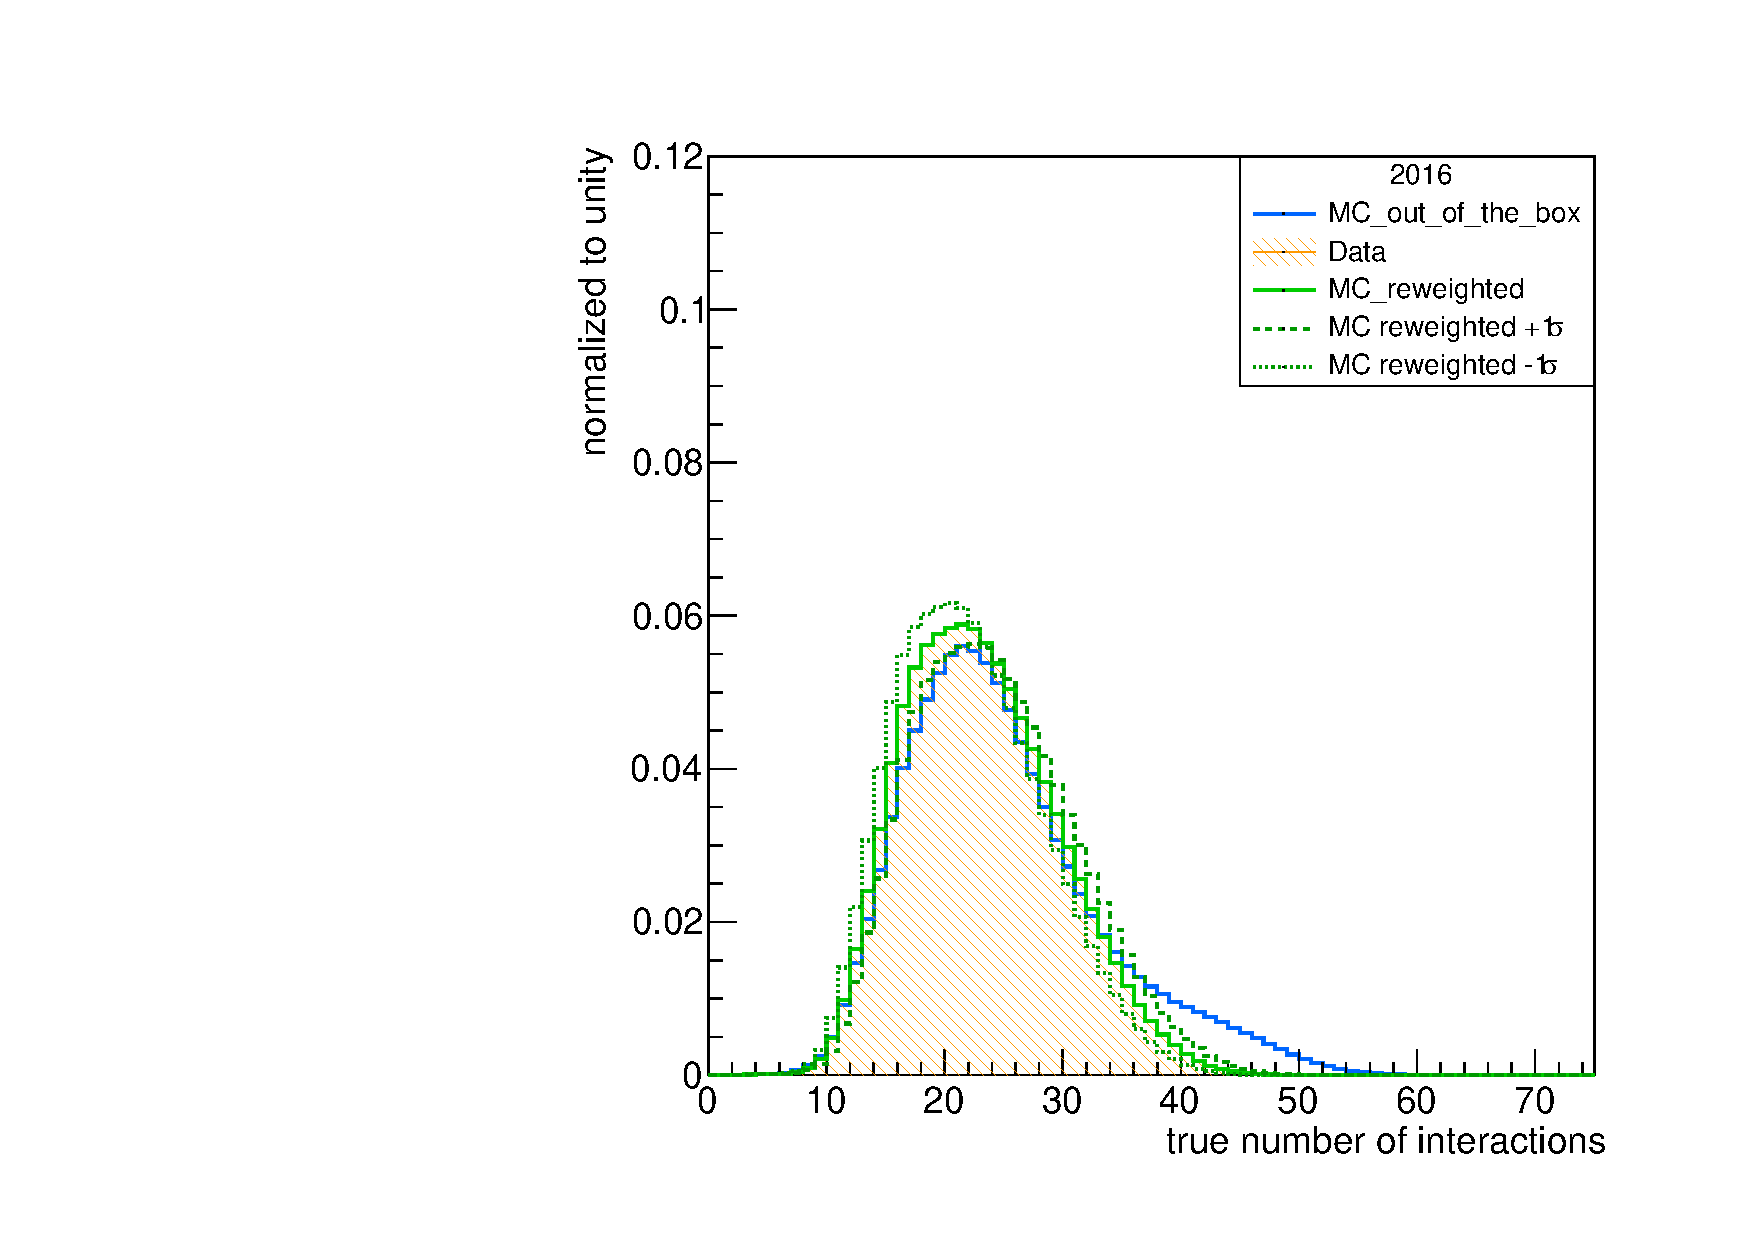
\includegraphics[width=0.45\textwidth]{Figures/PileUp/pu_weights_2016.pdf} \\
%                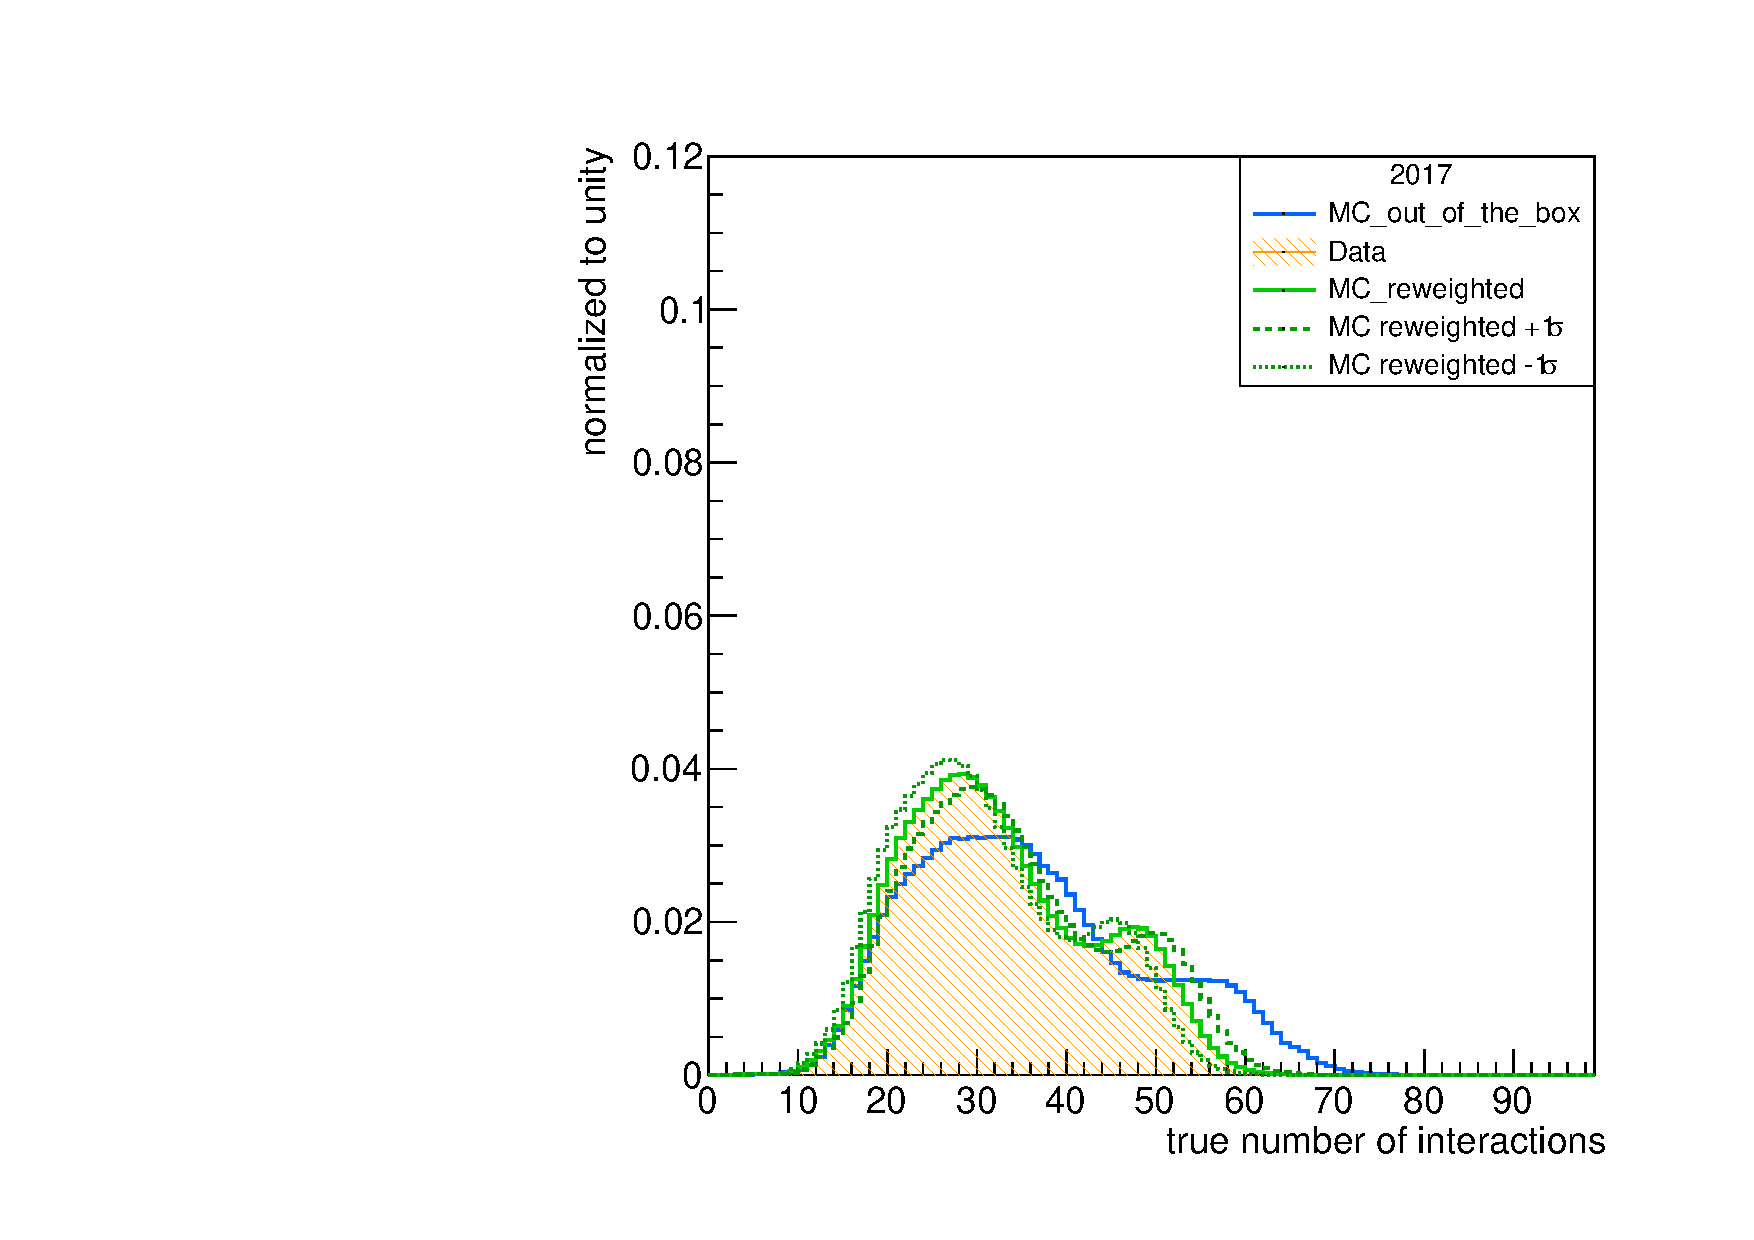
\includegraphics[width=0.45\textwidth]{Figures/PileUp/pu_weights_2017.pdf} \\
%                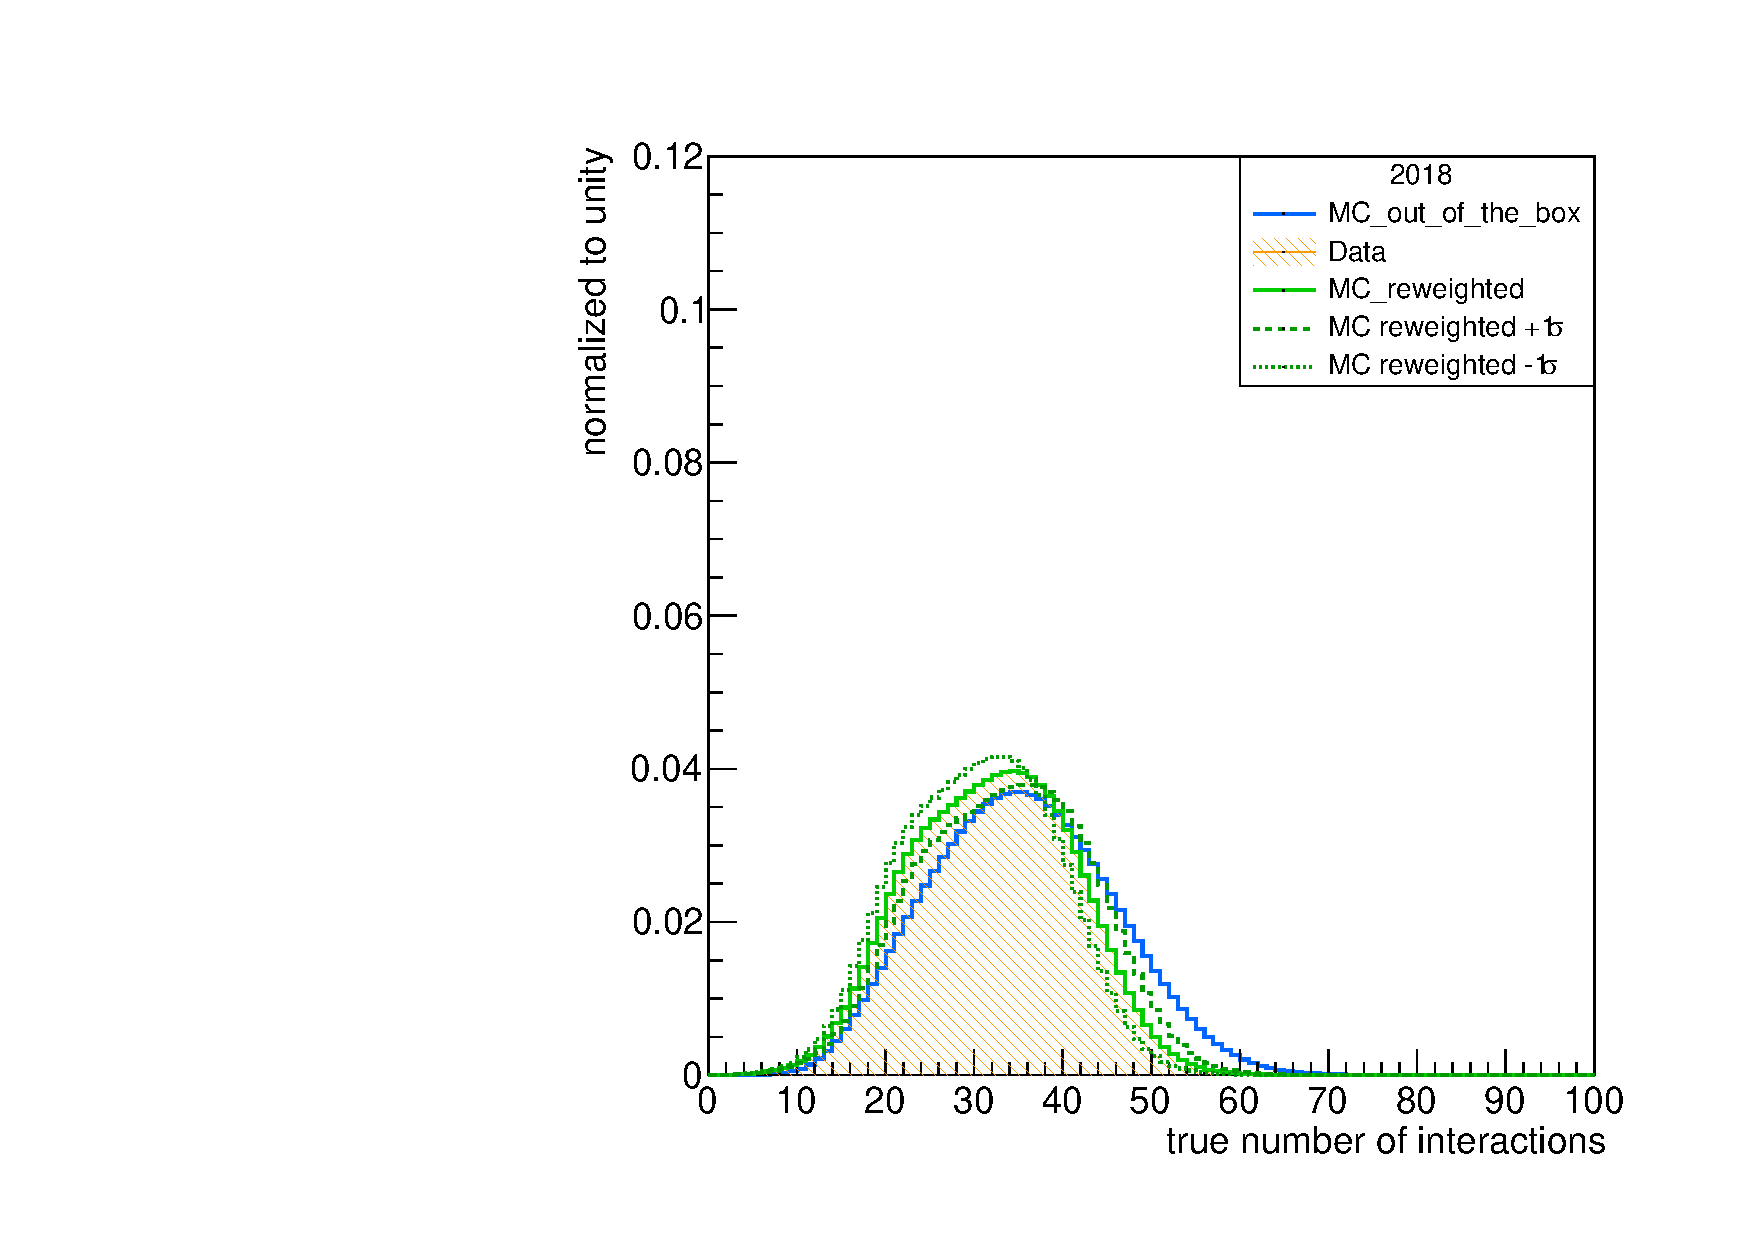
\includegraphics[width=0.45\textwidth]{Figures/PileUp/pu_weights_2018.pdf} \\
%		\caption{Distribution of pileup in 2016 (top), 2017 (middle) and 2018 (bottom) MC and Data shown before and after the application of PU weights. Up and down variations of 5\% in the minimum bias
%			cross section when calculating the weighs are also shown.
%			\label{fig:puWeight2018}}
%	\end{center}
%\end{figure}
%%=======

\subsection{Simulation samples for interpretations} \label{MCForInterpretations}
